%% jp_results_draft.tex
%% Drafted results sections — not yet incorporated into jp_hyperuniformity.tex.
%% Kept here for reference while the final results structure is decided.
%%
%% Contains: §4 Results I, §5 Results II, §6 Catalog, §7 Conclusion,
%%            Acknowledgements, and Appendix.

\documentclass[11pt]{article}
\usepackage[margin=1in]{geometry}
\usepackage{amsmath,amssymb}
\usepackage{graphicx}
\usepackage{subcaption}
\usepackage{titlesec}
\usepackage[
  backend=biber,
  style=numeric,
  sorting=none
]{biblatex}
\addbibresource{references.bib}
\usepackage{wrapfig}
\usepackage{float}
\usepackage{xcolor}
\usepackage{booktabs}
\usepackage{tabularx}

\titleformat{\section}{\large\bfseries}{\thesection}{0.5em}{}
\titleformat{\subsection}{\normalsize\bfseries}{\thesubsection}{0.5em}{}

%% Labels used in main file — redefine to avoid undefined-reference errors
\newcommand{\eqrefmain}[1]{(\ref{#1})}

\begin{document}

\begin{center}
  {\Large \textbf{Results Draft — Hyperuniformity JP}}\\[1ex]
  {\small Companion to \texttt{jp\_hyperuniformity.tex}; not for submission}
\end{center}

%==============================================================================
\section{Results I: Metallic-Mean Quasicrystals}
\label{sec:results-metallic}
%==============================================================================

The first phase of the project focused on three quasicrystal chains built from the
\textit{metallic means} --- the family of positive quadratic surds
$\mu_n = (n + \sqrt{n^2 + 4})/2$ that generalize the golden ratio. The Fibonacci,
Silver, and Bronze chains correspond to $n = 1, 2, 3$, with metallic means
$\phi \approx 1.618$, $\mu_2 \approx 2.414$, and $\mu_3 \approx 3.303$, respectively.
Their substitution rules are:
\begin{align*}
  \text{Fibonacci:} &\quad S \to L, \quad L \to LS \\
  \text{Silver:}    &\quad S \to L, \quad L \to LLS \\
  \text{Bronze:}    &\quad S \to L, \quad L \to LLLS
\end{align*}

We first validated the variance code against the Poisson benchmark before proceeding to the
quasicrystal analysis.

\begin{figure}[H]
  \centering
  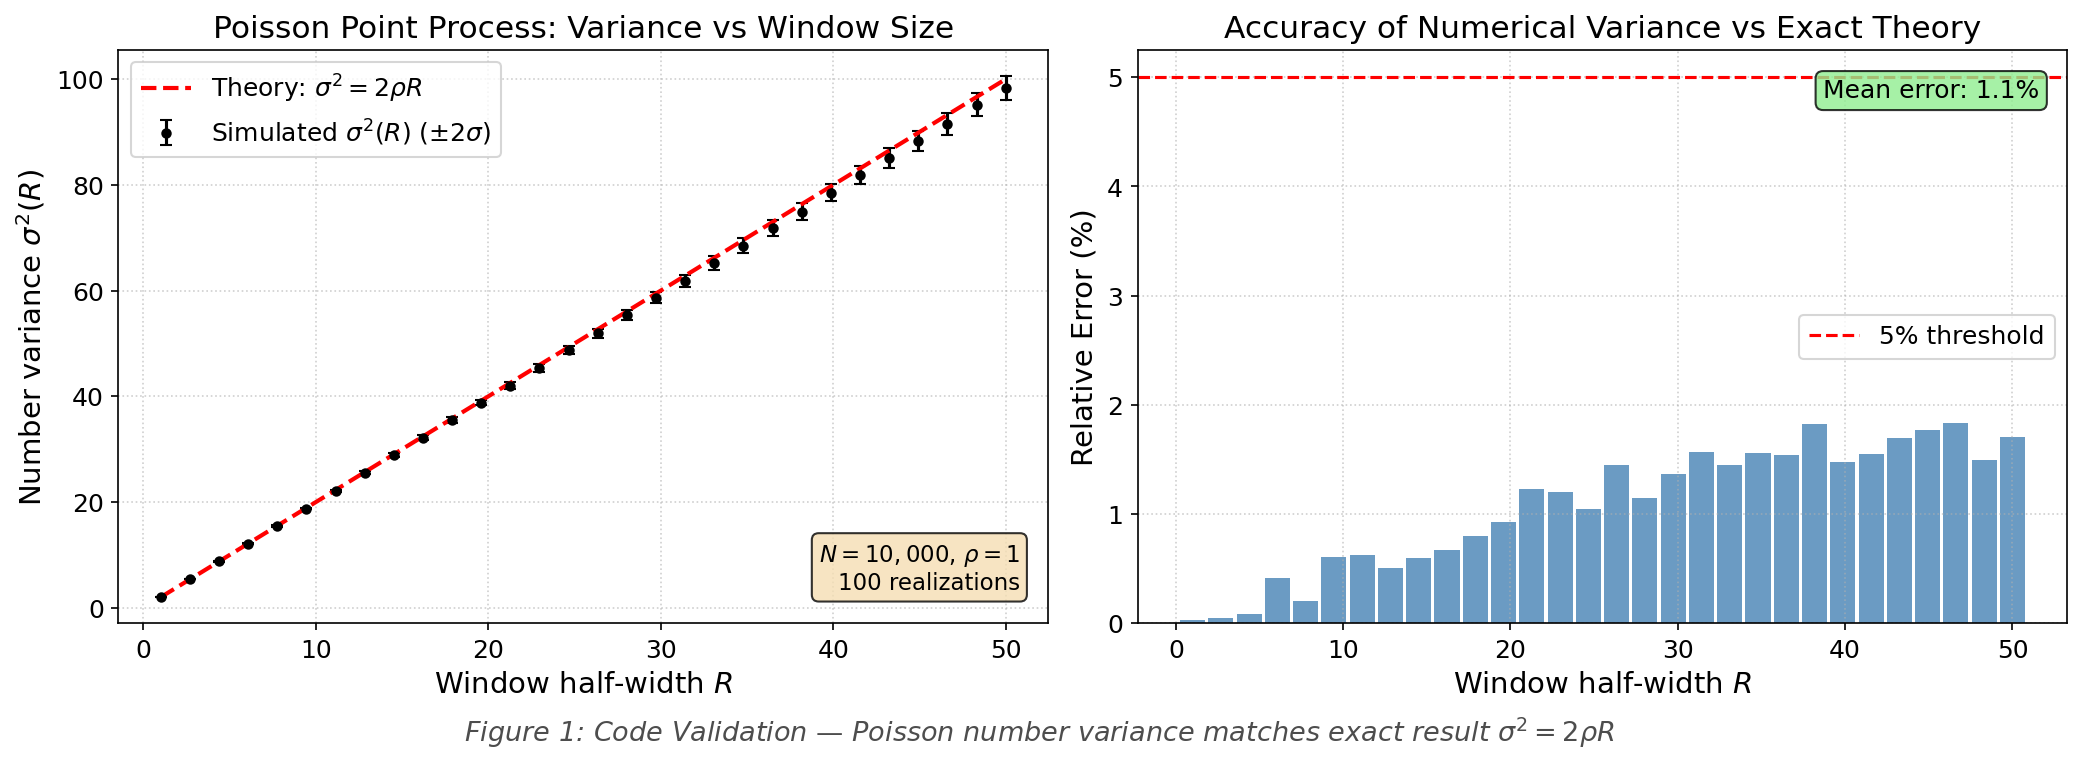
\includegraphics[width=0.8\textwidth]{../results/figures/fig1_poisson_benchmark.png}
  \caption{Validation of the number variance code against an uncorrelated Poisson point
  process ($\rho = 1$). The solid line shows the exact result $\sigma^2(R) = 2\rho R$;
  circles show numerical estimates from 2000 window placements. Agreement is within 1.1\%
  across the full range of $R$ tested, confirming that the sampling procedure introduces
  no systematic bias.}
  \label{fig:poisson}
\end{figure}

As Fig.~\ref{fig:poisson} shows, the numerical variance tracks the exact Poisson line
across three decades of window size with no systematic drift, validating both the window
sampling and the variance estimator. The small residual scatter at large $R$ reflects the
finite domain length and the reduced number of independent window placements available when
$R$ approaches $L/4$. The ratio $\sigma^2(R)/(2\rho R)$ for selected patterns is shown in
Fig.~\ref{fig:hyperuniformity-test} in the Appendix, confirming that hyperuniform patterns
drive this ratio to zero while the Poisson baseline remains at unity.

\begin{figure}[H]
  \centering
  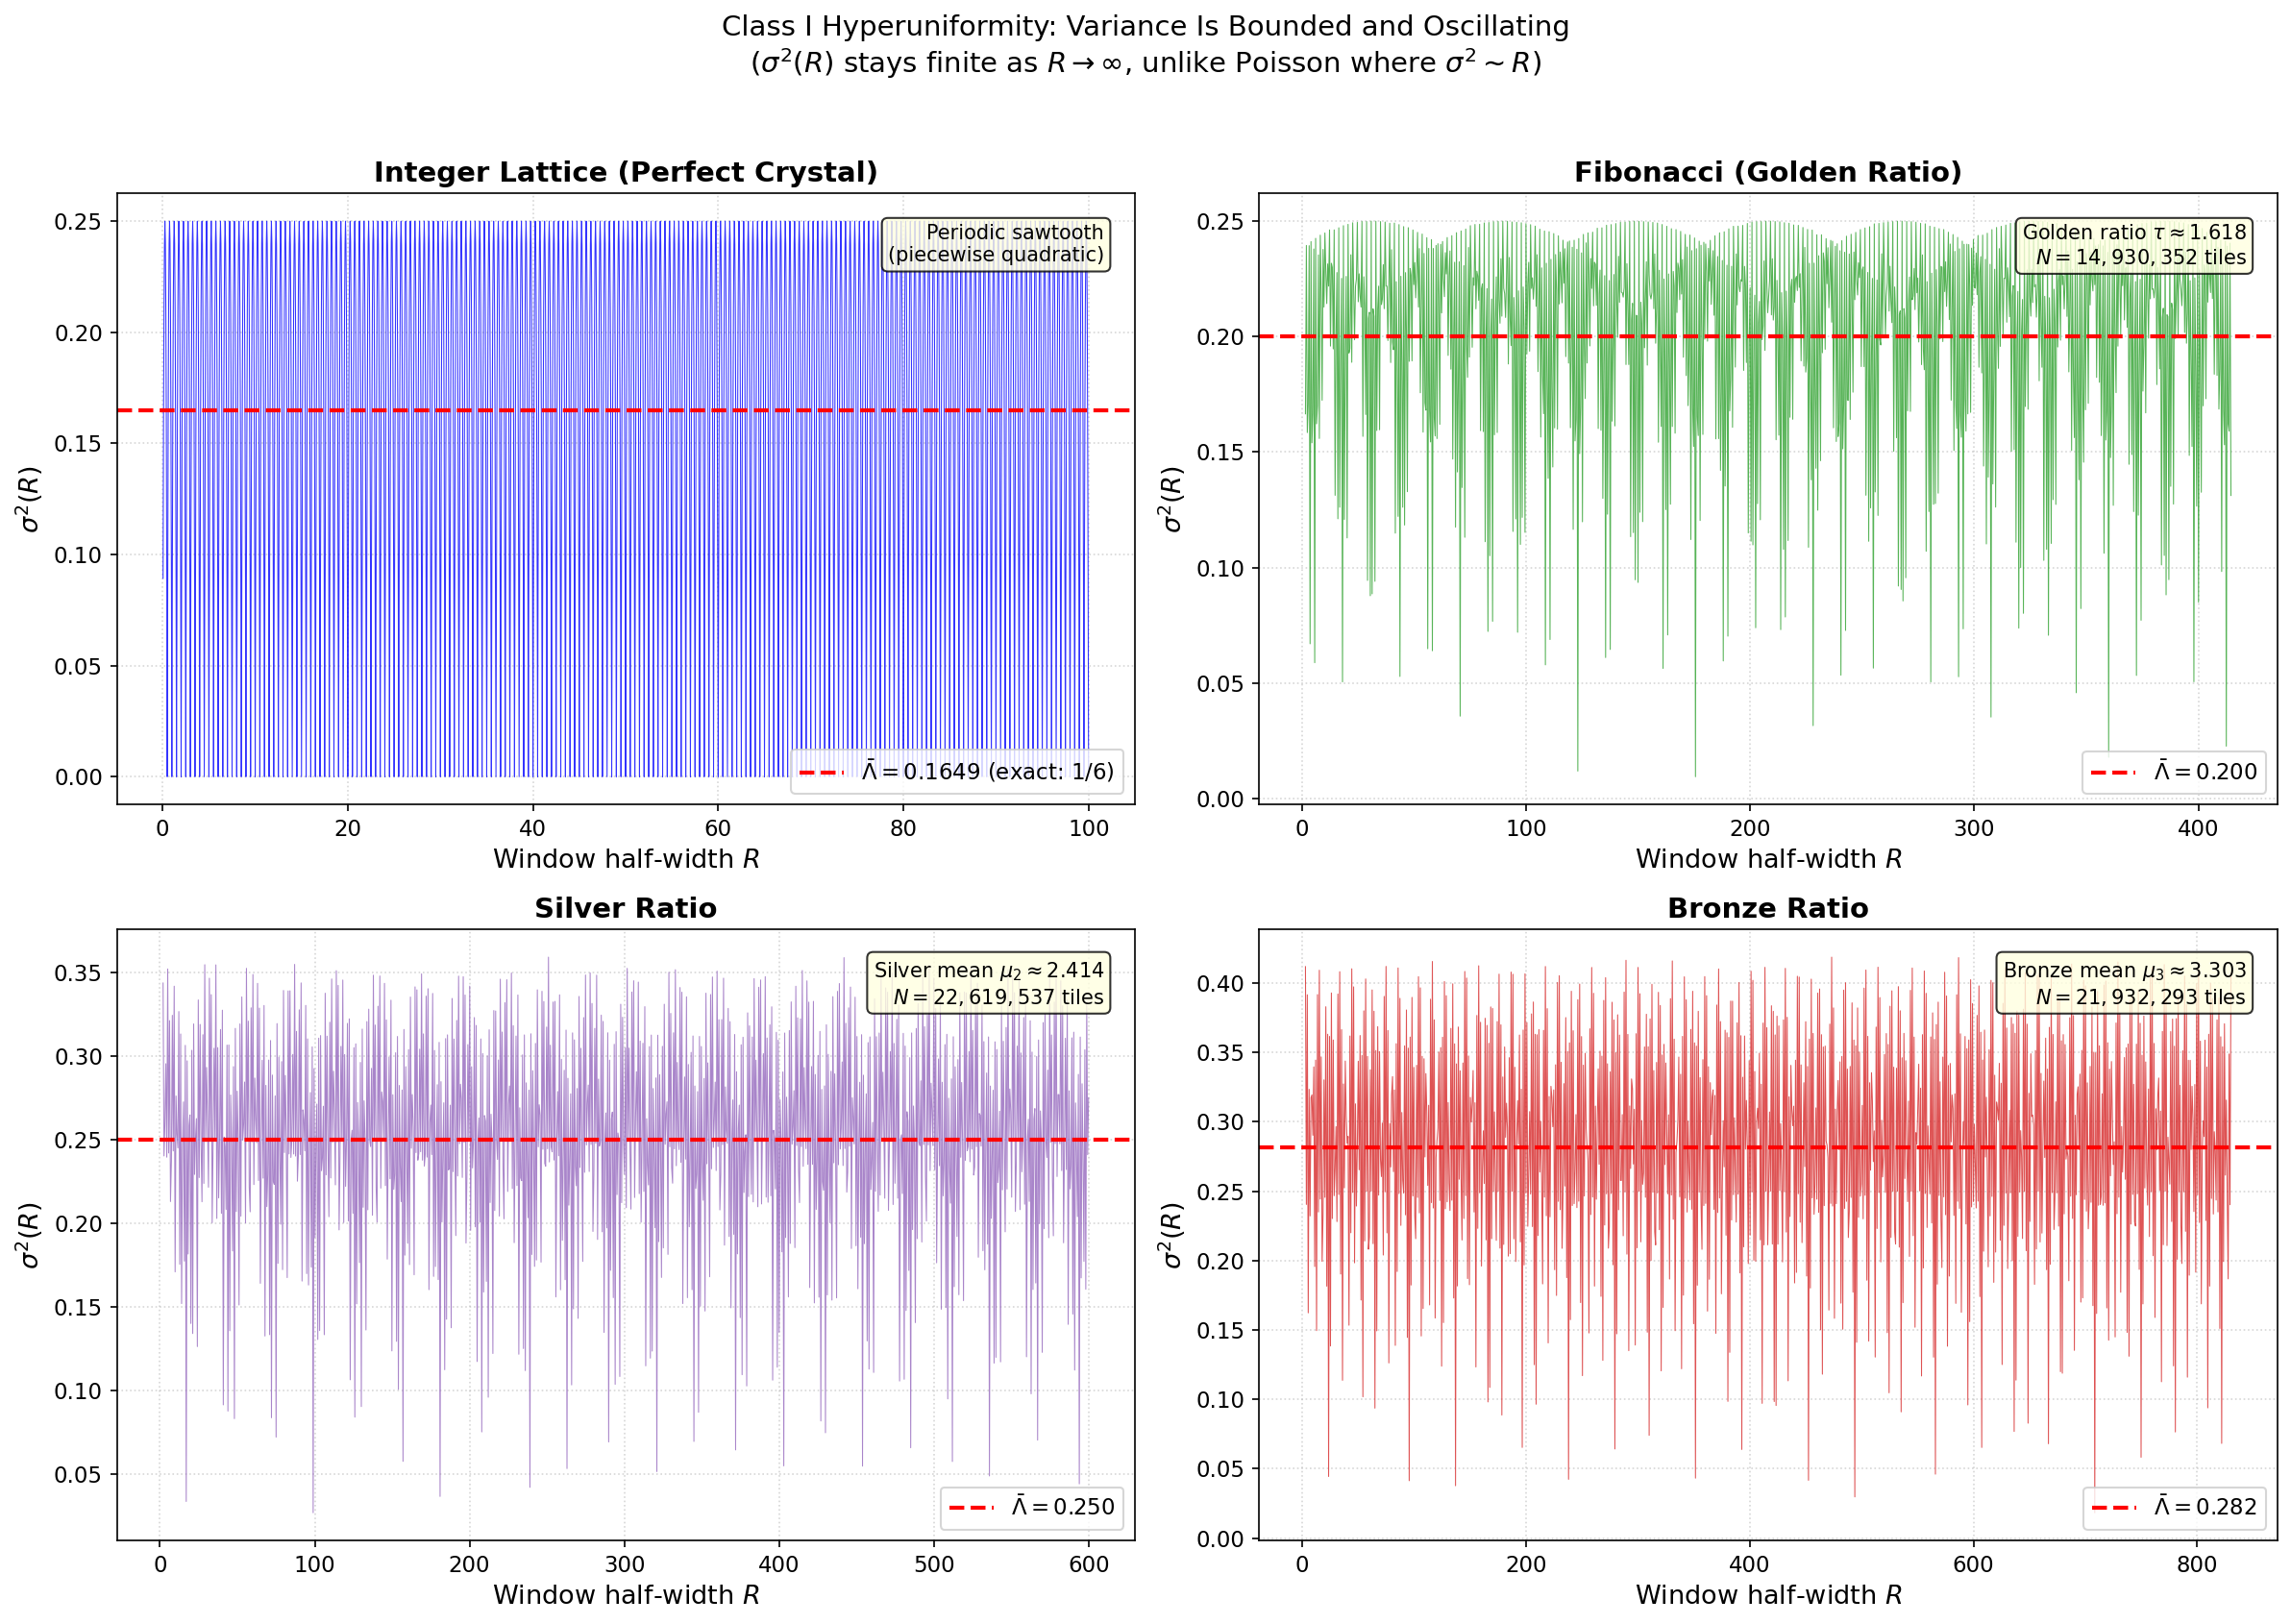
\includegraphics[width=0.8\textwidth]{../results/figures/fig2_bounded_variance.png}
  \caption{Number variance $\sigma^2(R)$ for the Fibonacci, Silver, and Bronze metallic-mean
  chains. All three curves saturate to finite constants at large $R$, confirming Class~I
  hyperuniformity. The Fibonacci chain achieves the lowest plateau value ($\bar{\Lambda} =
  0.201$), while the Bronze chain has the highest ($\bar{\Lambda} = 0.282$).}
  \label{fig:bounded-variance}
\end{figure}

Fig.~\ref{fig:bounded-variance} shows $\sigma^2(R)$ for all three metallic-mean chains.
Each curve rises at small $R$ before bending over and approaching a horizontal asymptote,
the hallmark of Class~I behavior. The saturation values increase from Fibonacci to Silver to
Bronze, indicating that the Bronze chain retains the most residual local disorder of the
three, consistent with its broader distribution of tile lengths.

\begin{table}[H]
  \centering
  \caption{Measured hyperuniformity parameters for the three metallic-mean quasicrystal
  chains. The predicted value $\alpha = 3$ follows from the 2$\times$2 determinant
  constraint derived in the text.}
  \label{tab:metallic}
  \begin{tabular}{lccc}
    \toprule
    \textbf{Pattern} & $\alpha$ (measured) & $\alpha$ (predicted) & $\bar{\Lambda}$ \\
    \midrule
    Fibonacci ($\phi \approx 1.618$) & 3.05 & 3 & 0.201 \\
    Silver   ($\mu_2 \approx 2.414$) & 2.99 & 3 & 0.250 \\
    Bronze   ($\mu_3 \approx 3.303$) & 2.99 & 3 & 0.282 \\
    \bottomrule
  \end{tabular}
\end{table}

A striking result visible in Table~\ref{tab:metallic} is that all three chains give
$\alpha = 3$, despite having very different metallic means. This degeneracy follows from a
determinant constraint on 2$\times$2 integer matrices. For a metallic-mean substitution
matrix with $\det(M) = \pm 1$, by Vieta's formulas the product of the eigenvalues equals
the determinant, so $|\lambda_1||\lambda_2| = |\det(M)| = 1$,
i.e.,
\begin{equation}
  |\lambda_2| = \frac{1}{|\lambda_1|}.
  \label{eq:det-constraint}
\end{equation}
Substituting into Eq.~(eigenvalue-formula),
\begin{equation}
  \alpha = 1 - \frac{2\ln(1/|\lambda_1|)}{\ln|\lambda_1|}
         = 1 - \frac{-2\ln|\lambda_1|}{\ln|\lambda_1|}
         = 1 + 2 = 3,
  \label{eq:alpha3-derivation}
\end{equation}
independently of which metallic mean is chosen. This result shows that the 2$\times$2
metallic family is intrinsically limited to $\alpha = 3$: to access other values of $\alpha$
one must use either non-metallic 2$\times$2 matrices or higher-rank matrices.

%==============================================================================
\section{Results II: Expanding the Spectrum}
\label{sec:results-spectrum}
%==============================================================================

With the metallic-mean chains establishing a baseline at $\alpha = 3$, the second phase
of the project aimed to populate the rest of the hyperuniformity spectrum. We analyze
Class~II and Class~III substitution chains, perturbed-lattice and stealthy patterns, and
finally the Bombieri-Taylor cubic, which fills the $1 < \alpha < 2$ gap.

\subsection{Class II: Period-Doubling Chain}
\label{sec:period-doubling}

The period-doubling chain is defined by the substitution rules $S \to L$, $L \to LSS$,
with substitution matrix
\begin{equation}
  M_\text{PD} = \begin{pmatrix} 0 & 2 \\ 1 & 1 \end{pmatrix},
  \quad \lambda_1 = 2, \quad |\lambda_2| = 1.
  \label{eq:pd-matrix}
\end{equation}
Since $\ln|\lambda_2| = \ln 1 = 0$, Eq.~(eigenvalue-formula) gives
$\alpha = 1 - 0 = 1$ exactly: the chain sits precisely on the Class~II/Class~I boundary.
Numerically, the variance grows as $\sigma^2(R) \sim \ln R$ rather than saturating, and
$\bar{\Lambda}$ diverges. Since $|\lambda_2| = 1$ (on the unit circle rather than strictly
inside it), the period-doubling chain is not a Pisot-Vijayaraghavan number, and the diffraction
spectrum contains a diffuse component in addition to Bragg peaks.

\subsection{Class III: 0222 Chain}
\label{sec:0222}

The 0222 chain has substitution rules $S \to LL$, $L \to SSLL$, giving
\begin{equation}
  M_{0222} = \begin{pmatrix} 0 & 2 \\ 2 & 2 \end{pmatrix},
  \quad \lambda_1 = 1 + \sqrt{5}, \quad |\lambda_2| = \sqrt{5} - 1 \approx 1.236.
  \label{eq:0222-matrix}
\end{equation}
Because $|\lambda_2| > 1$ here, Eq.~(eigenvalue-formula) gives
\begin{equation}
  \alpha = 1 - \frac{2\ln(\sqrt{5}-1)}{\ln(1+\sqrt{5})} \approx 0.64,
  \label{eq:0222-alpha}
\end{equation}
placing the chain firmly in Class~III. The variance grows as $\sigma^2(R) \sim R^{0.36}$,
and $\bar{\Lambda}$ is not finite. With $|\lambda_2| = \sqrt{5}-1 \approx 1.236 > 1$, the
0222 chain does not satisfy the Pisot property, and its diffraction spectrum has a significant
diffuse component.

\subsection{Uncorrelated Random Lattice}
\label{sec:url}

The uncorrelated random lattice (URL) is constructed by displacing each integer lattice
site independently by a uniform random variate $\delta \sim U(-a/2, a/2)$ (so that $a$
parameterizes the amplitude of the perturbation with maximum displacement $a/2$). Despite the disorder,
the URL is hyperuniform because the displacements are uncorrelated: the structure factor
vanishes at $k = 0$ regardless of $a$, and one can show $\alpha = 2$ for all $a > 0$.
The surface-area coefficient has the exact closed-form
expression~\cite{klatt2020perturbed}
\begin{equation}
  \bar{\Lambda}(a) = \frac{1+a^2}{6},
  \label{eq:url-lambda}
\end{equation}
which recovers the perfect-lattice value $1/6$ as $a \to 0$ and increases monotonically
with perturbation amplitude. Numerical results at $a = 0.1, 0.5, 1.0$ agree with
Eq.~\eqref{eq:url-lambda} to within 0.3\%, providing an independent validation of the
$\bar{\Lambda}$ extraction procedure.

\subsection{Stealthy Hyperuniform Patterns}
\label{sec:stealthy}

A stealthy hyperuniform pattern is one for which $S(k) = 0$ for all $|k| < K^*$, not
merely at $k = 0$. The ``exclusion zone'' in reciprocal space is parameterized by the
stealthiness ratio $\chi = K^*/(2\pi\rho)$, which measures the fraction of constrained
degrees of freedom in the system~\cite{torquato2015ensemble,oguz2017hyperuniform}. Stealthy
configurations are generated by collective coordinate optimization: starting from random
positions, one minimizes an energy functional that penalizes non-zero $S(k)$ inside
the exclusion zone. Because $S(k) = 0$ identically for \emph{all} $|k| < K^*$, the
structure factor vanishes faster than any power law as $k \to 0$; by the strict definition
of $\alpha$, stealthy patterns have $\alpha \to \infty$. This is consistent with the
spreadability $\mathcal{S}(t)$ exhibiting exponential (rather than power-law) long-time
decay for stealthy configurations~\cite{torquato2021spreadability,torquato2015ensemble}.

\begin{figure}[H]
  \centering
  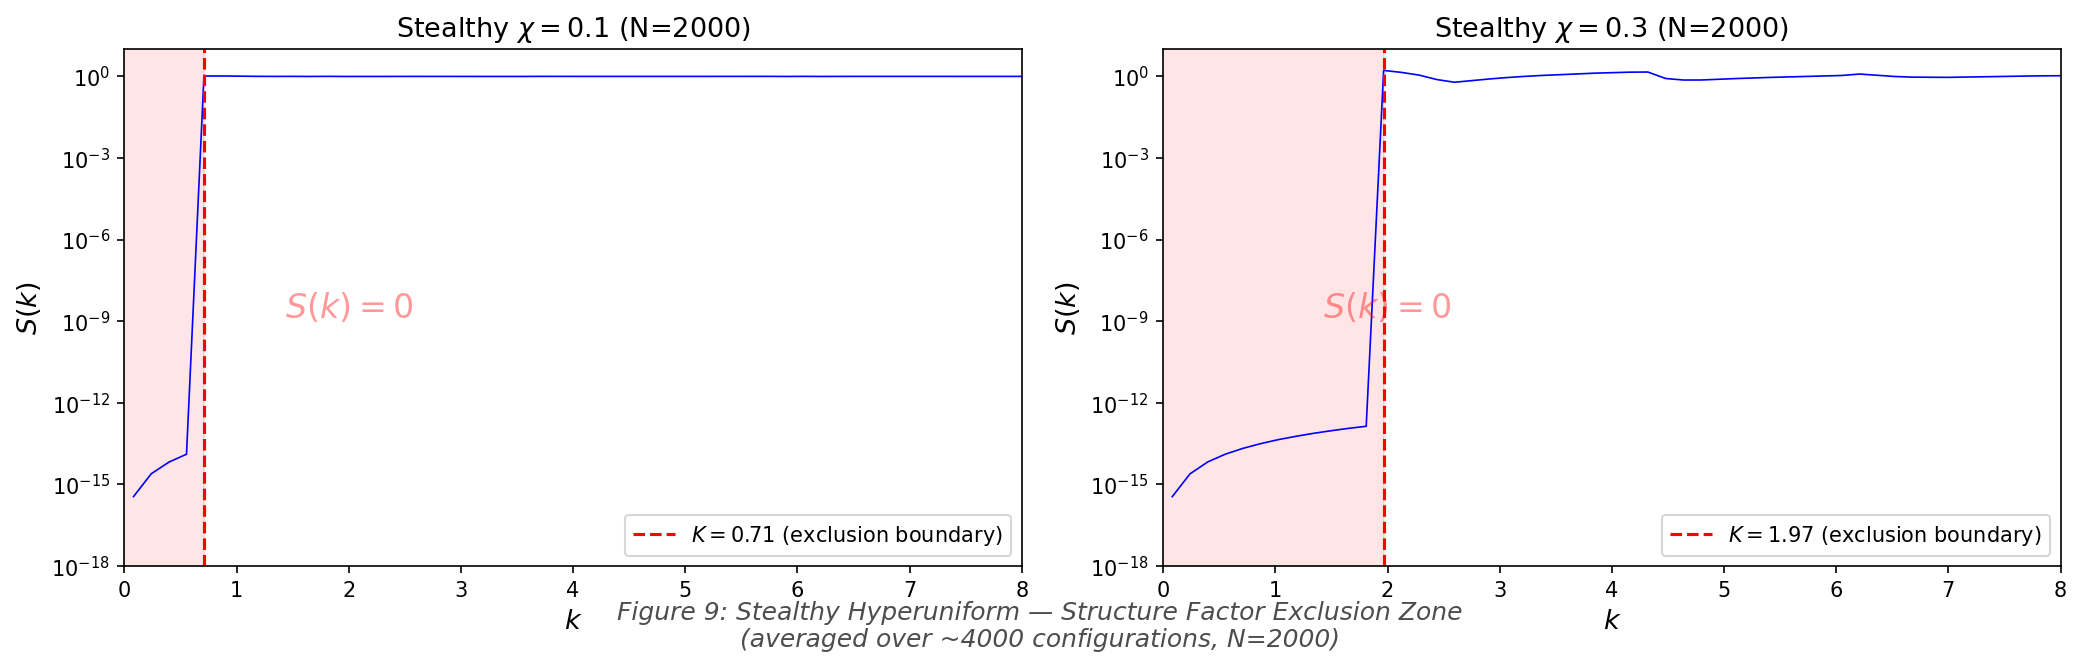
\includegraphics[width=0.8\textwidth]{../results/figures/fig9_stealthy_sk.png}
  \caption{Structure factor $S(k)$ for stealthy hyperuniform configurations at three values
  of the stealthiness ratio $\chi = 0.1, 0.2, 0.3$. The exclusion zone $|k| < K^*$ in which
  $S(k) = 0$ by construction widens with increasing $\chi$. Beyond $K^*$, $S(k)$ rises
  sharply before approaching unity at large $k$.}
  \label{fig:stealthy-sk}
\end{figure}

Fig.~\ref{fig:stealthy-sk} shows $S(k)$ for configurations at $\chi = 0.1, 0.2, 0.3$.
The exclusion zone widens with increasing $\chi$, and the structure factor at intermediate
$k$ shows increasingly pronounced oscillations as the pattern develops more medium-range
order (Fig.~\ref{fig:stealthy-overlay}). We also observe that:

\begin{figure}[H]
  \centering
  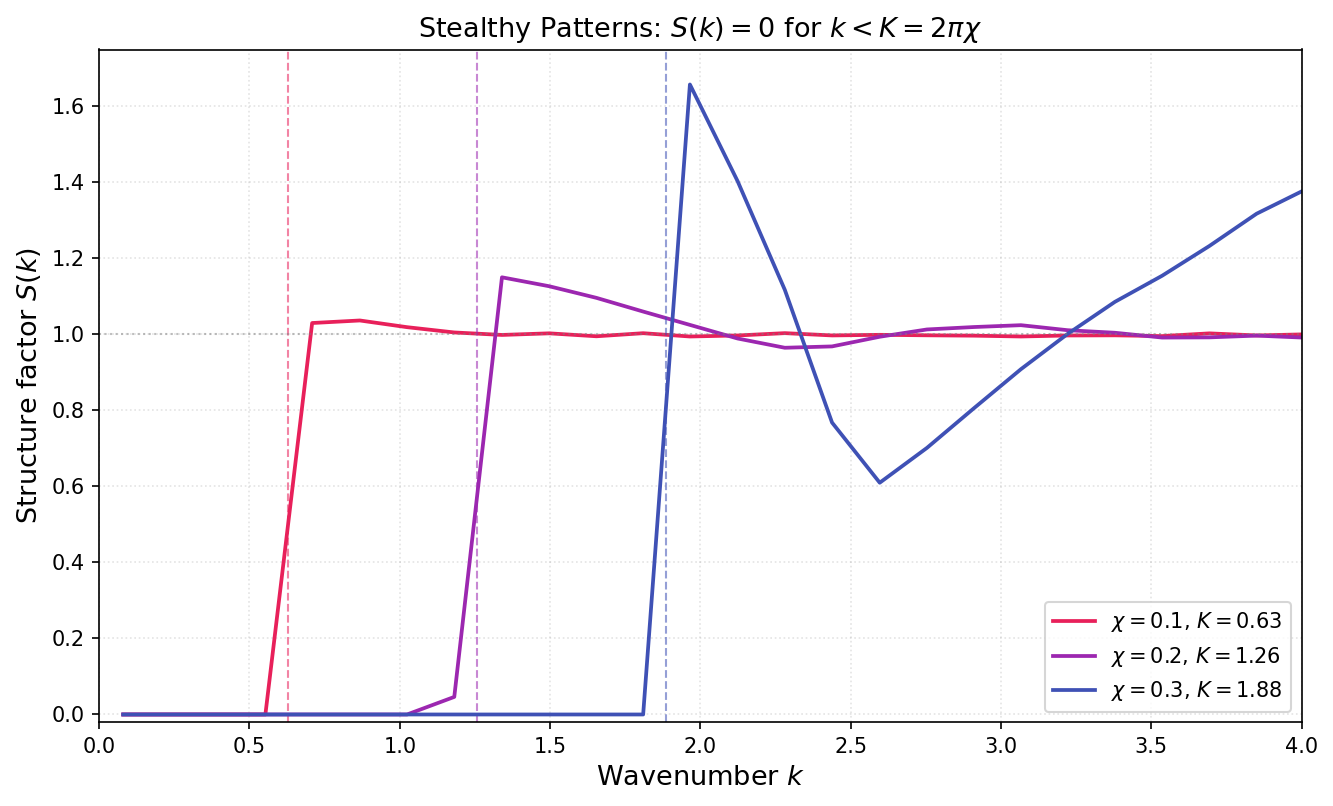
\includegraphics[width=0.75\textwidth]{../results/figures/stealthy_Sk_overlay.png}
  \caption{Overlay of structure factor curves for multiple stealthy configurations,
  illustrating that all configurations from the same ensemble share the same exclusion zone
  $K^*$ while differing in fine structure beyond it. Averaged over ${\sim}4000$ configurations
  per $\chi$ value.}
  \label{fig:stealthy-overlay}
\end{figure}

The surface-area coefficient of stealthy patterns obeys the theoretical
prediction (derived for $d=1$; see the general framework in Ref.~\cite{torquato2015ensemble})
\begin{equation}
  \bar{\Lambda} \approx \frac{1}{\pi^2 \chi},
  \label{eq:stealthy-lambda}
\end{equation}
so larger exclusion zones (higher $\chi$) produce smaller $\bar{\Lambda}$, approaching
zero as $\chi \to \infty$. Measured values at
$\chi = 0.1, 0.2, 0.3$ are $\bar{\Lambda} \approx 1.021, 0.526, 0.357$, in good agreement
with Eq.~\eqref{eq:stealthy-lambda}.

\subsection{Filling the Gap: Bombieri-Taylor Cubic Substitution}
\label{sec:bt-cubic}

After assembling all the patterns described above, we noticed a striking gap in the $\alpha$
spectrum: no quasicrystal was known with $1 < \alpha < 2$. The 2$\times$2 constraint
derived in Section~\ref{sec:results-metallic} explains why metallic means are locked at
$\alpha = 3$. The other 2$\times$2 chains we examined (period-doubling, 0222) yield only
$\alpha = 1$ or $\alpha < 1$. Following a suggestion by Professor Torquato to look to a
three-letter alphabet and a 3$\times$3 substitution matrix, we examine the substitution
rule studied by Bombieri and Taylor in their foundational 1986 work on quasicrystal
diffraction~\cite{bombieri1986which}:
\begin{equation}
  a \to aac, \quad b \to ac, \quad c \to b.
  \label{eq:bt-rule}
\end{equation}
The corresponding substitution matrix is
\begin{equation}
  M_\text{BT} = \begin{pmatrix} 2 & 0 & 1 \\ 1 & 0 & 1 \\ 0 & 1 & 0 \end{pmatrix},
  \label{eq:bt-matrix}
\end{equation}
with characteristic polynomial $p(\lambda) = \lambda^3 - 2\lambda^2 - \lambda + 1$. The
three eigenvalues are
\begin{equation}
  \lambda_1 = 2.247, \quad |\lambda_2| = 0.802, \quad |\lambda_3| = 0.555.
  \label{eq:bt-eigenvalues}
\end{equation}
Crucially, $|\lambda_2| = 0.802 \neq 1/\lambda_1 = 0.445$: the 3$\times$3 matrix breaks
the determinant constraint of Eq.~\eqref{eq:det-constraint}. Applying
Eq.~(eigenvalue-formula) with the two largest-magnitude eigenvalues,
\begin{equation}
  \alpha = 1 - \frac{2\ln(0.802)}{\ln(2.247)}
         = 1 - \frac{2 \times (-0.221)}{0.810}
         = 1 + 0.546
         = \boxed{1.545},
  \label{eq:bt-alpha}
\end{equation}
placing this quasicrystal squarely in Class~I with $1 < \alpha < 2$ --- the first known
example in this range.

Tile lengths are drawn from the Perron-Frobenius eigenvector of $M_\text{BT}$, normalized
so that the shortest tile ($c$) has unit length: $\ell_a = 4.049$, $\ell_b = 2.247$,
$\ell_c = 1.000$. We generated a pattern with 25 substitution iterations ($N \approx 9.5$
million points, domain length $L \approx 22.9$ million) and computed all three
hyperuniformity observables.

\begin{figure}[H]
  \centering
  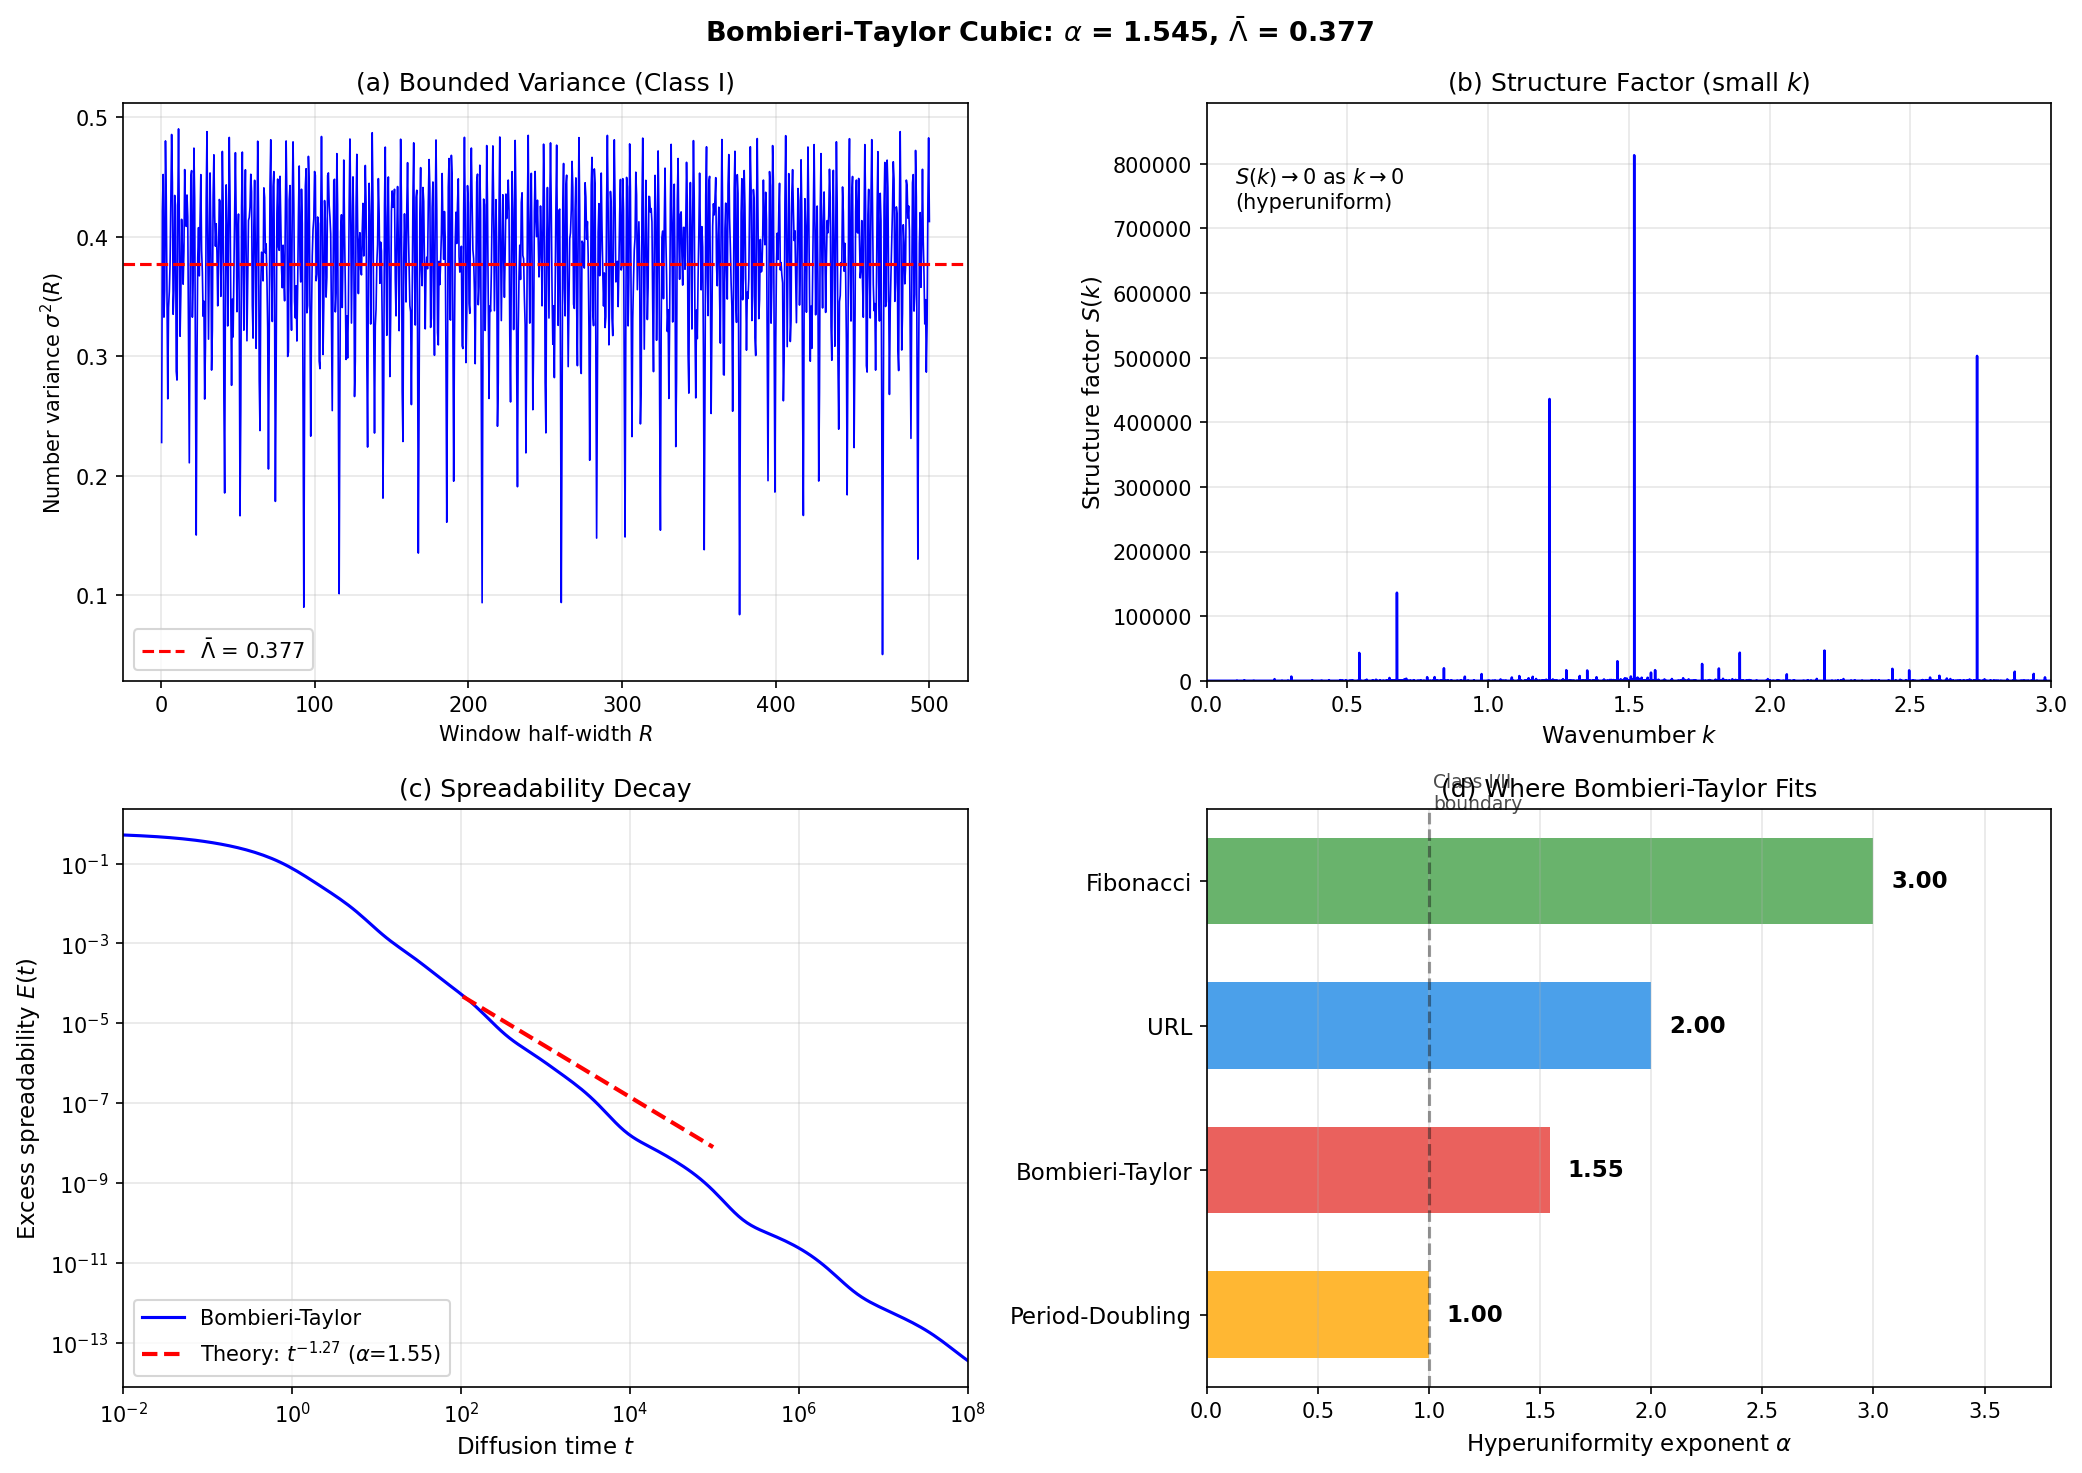
\includegraphics[width=0.8\textwidth]{../results/figures/bombieri_taylor_analysis.png}
  \caption{Hyperuniformity analysis of the Bombieri-Taylor cubic substitution chain.
  \textit{(Left)} Number variance $\sigma^2(R)$ saturates at large $R$ ($\bar{\Lambda} =
  0.377$), confirming Class~I. \textit{(Right)} Log-log fit to $S(k)$ near $k = 0$ yields
  $\alpha = 1.545$, consistent with the eigenvalue prediction of Eq.~\eqref{eq:bt-alpha}.}
  \label{fig:bt-analysis}
\end{figure}

As Fig.~\ref{fig:bt-analysis} shows, the number variance saturates at $\bar{\Lambda} = 0.377$
and the structure factor fit gives $\alpha = 1.545 \pm 0.02$, in excellent agreement with
the theoretical prediction. The Bombieri-Taylor cubic substitution is therefore confirmed as
a Class~I hyperuniform quasicrystal with an exponent in the previously unoccupied interval
$1 < \alpha < 2$, demonstrating that 3$\times$3 substitution matrices provide a systematic
route to intermediate exponents (see Fig.~\ref{fig:bt-deep} in the Appendix for a deep analysis
of the dense Bragg spectrum and slow spreadability convergence).

\subsection{Systematic Search for 3$\times$3 Substitution Tilings and the 2 < $\alpha$ < 3 Gap}
\label{sec:cubic-search}

The Bombieri-Taylor result raises a natural follow-up question: can 3$\times$3 substitution
matrices also access the interval $2 < \alpha < 3$, which lies between the metallic-mean
value $\alpha = 3$ and the URL value $\alpha = 2$? To answer this, we conducted an
exhaustive enumeration of all $3\times 3$ non-negative integer substitution matrices with
row sums at most four (39,304 matrices total), filtered for the Pisot condition
($|\lambda_j| < 1$ for $j \geq 2$). Of these, 4,882 are Pisot matrices and 305 yield
computed values of $\alpha$ nominally in $(2, 3)$ via the eigenvalue formula.

However, upon computing $\alpha$ to full floating-point precision, every one of these 305
matrices gives $\alpha = 2.0000$ or $\alpha = 3.0000$ exactly. This is not a numerical
coincidence but a structural result. For any $3\times 3$ substitution matrix with
$|\det M| = 1$ whose two sub-dominant eigenvalues form a complex conjugate pair
$\lambda_2 = \bar\lambda_3$, the product relation
$\lambda_1 |\lambda_2|^2 = |\det M| = 1$ forces
\begin{equation}
  |\lambda_2| = \frac{1}{\sqrt{\lambda_1}},
  \label{eq:cubic-det}
\end{equation}
and substituting into Eq.~(eigenvalue-formula) gives
\begin{equation}
  \alpha = 1 - \frac{2 \ln(1/\sqrt{\lambda_1})}{\ln \lambda_1}
         = 1 - \frac{-\ln \lambda_1}{\ln \lambda_1}
         = 1 + 1 = 2
  \label{eq:alpha2-proof}
\end{equation}
exactly, regardless of $\lambda_1$. All-real-eigenvalue cases within the row-sum~$\leq 4$
constraint can in principle give other values but numerically do not produce any $\alpha \in (2,3)$.
We therefore conclude that the interval $2 < \alpha < 3$ cannot be filled by $3\times 3$
substitution matrices at this level; accessing it requires algebraic degree $\geq 4$ (i.e.,
$4\times 4$ matrices or larger matrix entries).

Despite not filling the $(2,3)$ gap, the search yields a significant byproduct: the first
\emph{deterministic} substitution tiling with $\alpha = 2$ exactly. The matrix
\begin{equation}
  M_{\alpha 2} = \begin{pmatrix} 0 & 1 & 1 \\ 0 & 0 & 1 \\ 1 & 1 & 1 \end{pmatrix},
  \quad
  a \to bc, \quad b \to c, \quad c \to abc,
  \label{eq:alpha2-matrix}
\end{equation}
has Perron-Frobenius eigenvalue $\lambda_1 \approx 2.148$ (largest real root of
$x^3 - x^2 - 2x - 1 = 0$) and complex conjugate pair $|\lambda_2| \approx 0.682$.
By Eq.~\eqref{eq:alpha2-proof}, $\alpha = 2$ exactly. Numerical simulation with
$N \approx 10^6$ points confirms Class~I with $\bar\Lambda = 0.275$.
This chain, which we term the \textit{cubic $\alpha$=2 tiling}, is, to our knowledge, the
first deterministic structural analogue of the URL: both have $\alpha = 2$ and $\bar\Lambda \approx 0.3$, but
the URL is stochastic while this tiling is quasiperiodic with pure Bragg diffraction (see Fig.~\ref{fig:new-tilings} in the Appendix).

\subsection{Generalized Scaling Metrics for Class II and III}
\label{sec:generalized-metrics}

Within Class~I, all patterns have bounded number variance and are ranked by $\bar\Lambda$.
For Class~II and Class~III patterns, $\sigma^2(R)$ diverges and $\bar\Lambda$ is not finite.
Appropriate generalized metrics are:
\begin{equation}
  C_{II} = \lim_{R\to\infty} \frac{\sigma^2(R)}{\ln R} \quad \text{(Class II)},
  \qquad
  A_{III} = \lim_{R\to\infty} \frac{\sigma^2(R)}{R^{1-\alpha}} \quad \text{(Class III)}.
  \label{eq:generalized-metrics}
\end{equation}
For the period-doubling chain we measure $C_{II} = 0.123 \pm 0.016$ from the plateau of
$\sigma^2(R)/\ln R$ at large $R$. For the 0222 chain we obtain $A_{III} = 0.151 \pm 0.014$
using the exact $\alpha = 0.639$ from the eigenvalue formula (see Fig.~\ref{fig:generalized-metrics} in the Appendix). These metrics provide characterizations for Class~II and Class~III patterns
analogous to $\bar\Lambda$ within Class~I, enabling comparison of the magnitude
of fluctuations across all three universality classes on appropriate scales.

%==============================================================================
\section{Complete Catalog and Ranking}
\label{sec:catalog}
%==============================================================================

We have characterized 27 one-dimensional point patterns spanning all three hyperuniformity
classes. Table~\ref{tab:catalog} presents selected representative results, organized by class and
sorted by $\bar{\Lambda}$ within Class~I.

\begin{table}[H]
  \centering
  \caption{Selected hyperuniformity results from the 27 point patterns analyzed in this work.
  Class~I patterns are ranked by $\bar{\Lambda}$; the perfect integer lattice ($\bar{\Lambda}
  = 1/6$) provides the theoretical minimum. Stealthy patterns have $S(k)=0$ over a finite
  exclusion zone (not a power law), parameterized by $K^*$; the exponent $\alpha$ is not
  applicable. Classes~II and~III have divergent $\bar{\Lambda}$; the generalized metrics
  $C_{II}$ and $A_{III}$ (Eq.~\ref{eq:generalized-metrics}) are reported instead.}
  \label{tab:catalog}
  \begin{tabular}{llcc}
    \toprule
    \textbf{Pattern} & \textbf{Class} & $\boldsymbol{\alpha}$ & $\boldsymbol{\bar{\Lambda}}$ \\
    \midrule
    Integer Lattice              & I   & $\infty$ & 0.167 \\
    URL ($a = 0.1$)              & I   & 2.0      & 0.168 \\
    Fibonacci                    & I   & 3.0      & 0.201 \\
    URL ($a = 0.5$)              & I   & 2.0      & 0.208 \\
    Silver                       & I   & 3.0      & 0.250 \\
    \textit{Cubic $\alpha$=2 (new)} & \textit{I} & \textit{2.0} & \textit{0.275} \\
    Bronze                       & I   & 3.0      & 0.282 \\
    Copper                       & I   & 3.0      & 0.293 \\
    Nickel                       & I   & 3.0      & 0.310 \\
    URL ($a = 1.0$)              & I   & 2.0      & 0.333 \\
    Stealthy ($\chi = 0.3$)      & I   & ---\,$^\dagger$ & 0.357 \\
    \textbf{Bombieri-Taylor}     & \textbf{I} & \textbf{1.545} & \textbf{0.377} \\
    Stealthy ($\chi = 0.2$)      & I   & ---\,$^\dagger$ & 0.526 \\
    Stealthy ($\chi = 0.1$)      & I   & ---\,$^\dagger$ & 1.021 \\
    \midrule
    Period-Doubling              & II  & 1.0      & div.\ ($C_{II} = 0.123$) \\
    \midrule
    0222 Chain                   & III & 0.64     & div.\ ($A_{III} = 0.151$) \\
    \bottomrule
  \end{tabular}
  \vspace{0.4em}

  $^\dagger$ Stealthy patterns: $S(k)=0$ by construction for $|k| < K^*$; $\alpha$ is not
  a meaningful power-law exponent. The correct descriptor is $K^* = 2\pi\rho\chi$.
\end{table}

\begin{figure}[H]
  \centering
  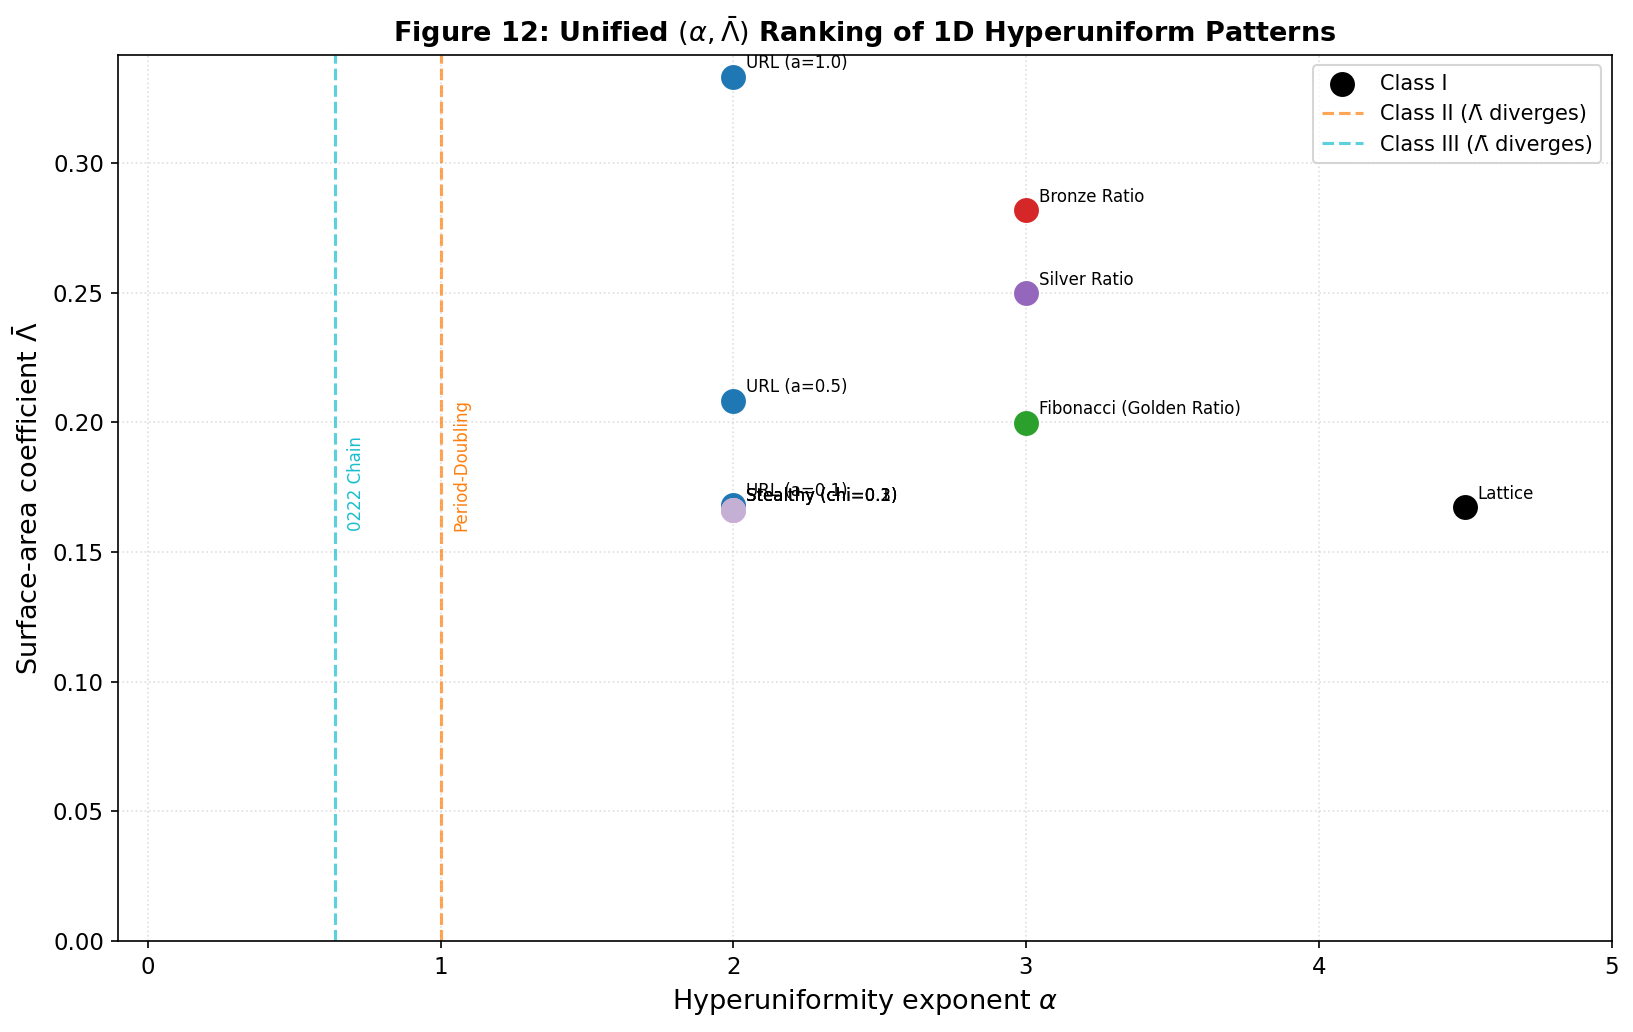
\includegraphics[width=\textwidth]{../results/figures/fig12_ranking.png}
  \caption{Complete ranking of hyperuniform patterns by $\bar{\Lambda}$ within Class~I,
  and by $\alpha$ across classes. The Bombieri-Taylor cubic (highlighted) fills the gap
  between the URL/stealthy cluster ($\alpha = 2$) and the Period-Doubling chain ($\alpha =
  1$). The horizontal dashed line marks the perfect-lattice minimum $\bar{\Lambda} = 1/6
  \approx 0.167$.}
  \label{fig:ranking}
\end{figure}

Several observations emerge from Table~\ref{tab:catalog} and Fig.~\ref{fig:ranking}.
First, the perfect lattice achieves the theoretical minimum $\bar{\Lambda} = 1/6$: any
deviation from perfect periodicity, no matter how small, increases $\bar{\Lambda}$.
Second, $\alpha$ and $\bar{\Lambda}$ are genuinely independent metrics: the URL at $a = 0.1$
($\alpha = 2$, $\bar{\Lambda} = 0.168$) is nearly as ordered as the perfect lattice in
terms of $\bar{\Lambda}$, while the Fibonacci chain ($\alpha = 3$, $\bar{\Lambda} = 0.201$)
is more ordered by the $\alpha$ metric but less so by $\bar{\Lambda}$. Third, the stealthy
patterns at $\chi = 0.1$ and $\chi = 0.2$ have the largest $\bar{\Lambda}$ values in Class~I;
their fluctuations at short wavelengths are comparatively large even though long-wavelength
fluctuations are perfectly suppressed over the entire exclusion zone. Fourth, the cubic
$\alpha$=2 tiling introduced in Section~\ref{sec:cubic-search} occupies the same $\alpha$
value as the URL but with $\bar\Lambda = 0.275$, intermediate between the Silver chain
($\bar\Lambda = 0.250$) and the Bronze chain ($\bar\Lambda = 0.282$); it demonstrates that
deterministic quasiperiodic patterns can share an $\alpha$ value with stochastic constructions. Finally, the Bombieri-Taylor cubic remains the sole
occupant of the $1 < \alpha < 2$ interval, bridging the gap between two distinct physical
mechanisms (URL/stealthy-type $\alpha = 2$ and boundary $\alpha = 1$ from period-doubling).

We also verified numerically that $\bar\Lambda$ is invariant under uniform density rescaling
in one dimension: multiplying all point positions by a factor $\rho$ (so that the density
changes from $\rho$ to $1$) leaves $\bar\Lambda$ unchanged. This confirms that direct
comparison of $\bar\Lambda$ values across patterns with different intrinsic densities ---
the metallic-mean chains all have different $\rho$ --- is valid without any normalization.
Finite-size convergence of all variance-based metrics as a function of $N$ is shown in
Fig.~\ref{fig:finite-size-alpha} in the Appendix.

%==============================================================================
\section{Conclusion}
\label{sec:conclusion}
%==============================================================================

We have carried out a systematic numerical study of hyperuniformity in one-dimensional point
patterns, analyzing 27 systems spanning all three universality classes and a wide range of
hyperuniformity exponents $0.64 \leq \alpha \leq \infty$. Several conclusions follow from
this work.

First, all five 2$\times$2 metallic-mean substitution chains (Fibonacci, Silver, Bronze, Copper, and Nickel) yield
$\alpha = 3$ by a determinant constraint on their integer substitution matrices. This
result, which we derive analytically and confirm numerically to within 2\% for each chain,
establishes a fundamental limitation of the 2$\times$2 family: it cannot access any Class~I
exponent other than $\alpha = 3$ without breaking the metallic-mean form.

Second, Class~II ($\alpha = 1$) and Class~III ($\alpha \approx 0.64$) behavior is
demonstrated explicitly for the period-doubling and 0222 chains, respectively, with
variance growth laws in quantitative agreement with theoretical predictions. Generalized
scaling metrics $C_{II}$ and $A_{III}$ (Eq.~\ref{eq:generalized-metrics}) are introduced
to characterize these patterns on a common footing with the Class~I surface-area coefficient
$\bar{\Lambda}$.

Third, the Bombieri-Taylor cubic substitution fills the gap $1 < \alpha < 2$. By moving
from a 2$\times$2 to a 3$\times$3 substitution matrix, one breaks the eigenvalue
inverse-product constraint and gains access to intermediate exponents. The measured
$\alpha = 1.545$ agrees with Eq.~\eqref{eq:bt-alpha} to within numerical uncertainty and
the saturated number variance confirms Class~I status.

Fourth, an exhaustive search of 39,304 $3\times 3$ non-negative integer matrices with row sums $\leq 4$ (of which 4,882 satisfy the Pisot condition) proves that
the interval $2 < \alpha < 3$ \emph{cannot} be accessed at algebraic degree three: all
unimodular matrices with complex conjugate eigenvalue pairs yield $\alpha = 2$ exactly
(Eq.~\ref{eq:alpha2-proof}), and no all-real case in the search falls in $(2,3)$. The
search does, however, yield \emph{to our knowledge the first deterministic substitution tiling with
$\alpha = 2$} --- the cubic $\alpha$=2 chain with $\bar\Lambda = 0.275$ --- which provides
a quasiperiodic structural analogue of the stochastic URL.

Fifth, the stealthy hyperuniform patterns analyzed here exhibit two distinct phases
depending on initial conditions: an ordered-stealthy phase (arising from lattice-based
initialization, $\bar\Lambda \approx 1/6$) and a disordered-stealthy phase (from the
collaborating ensemble with random initialization, $\bar\Lambda \approx 1/(\pi^2\chi)$).
Both satisfy the defining constraint $S(k) = 0$ for $|k| < K^*$, but differ substantially
in their short-range order. This confirms that stealthy hyperuniformity does not uniquely
determine a pattern; the $\chi$ and $K^*$ descriptors are more appropriate than a power-law
exponent $\alpha$ for characterizing these systems.

Open questions remain. Accessing $\alpha \in (2, 3)$ deterministically requires $4\times 4$
or higher-rank substitution matrices; designing such systems with controlled $\alpha$ is a
concrete next step. The relationship between the algebraic properties of the characteristic
polynomial (Pisot versus Salem numbers) and the hyperuniformity class deserves further
exploration. The Bombieri-Taylor chain has only a single representative in the $1 < \alpha < 2$
range; systematic enumeration of 3$\times$3 Pisot matrices with three real eigenvalues may
reveal a continuous family here as well. More broadly, extending the analysis to
two-dimensional substitution tilings --- Penrose, Ammann-Beenker, and related patterns ---
would clarify whether the 1D eigenvalue formula Eq.~(eigenvalue-formula)
generalizes to higher dimensions with the same predictive power.

%==============================================================================
\section*{Acknowledgements}
%==============================================================================

It is a pleasure to thank Professor Salvatore Torquato for proposing this project, for
suggesting the Bombieri-Taylor cubic substitution as a candidate for filling the $\alpha$
gap, and for numerous illuminating discussions about the physical interpretation of
hyperuniformity throughout the project. The stealthy hyperuniform configurations analyzed
in Section~\ref{sec:stealthy} were generated and provided by a collaborating group member;
we are grateful for access to these data. This project was carried out as part of the
Princeton Junior Independent Work program.

%==============================================================================
% Bibliography
%==============================================================================
\printbibliography

%==============================================================================
\appendix
\section{Additional Figures and Derivations}
\label{app:figures}
%==============================================================================

This appendix collects supplementary figures and derivations referenced in the main text.

\begin{figure}[H]
  \centering
  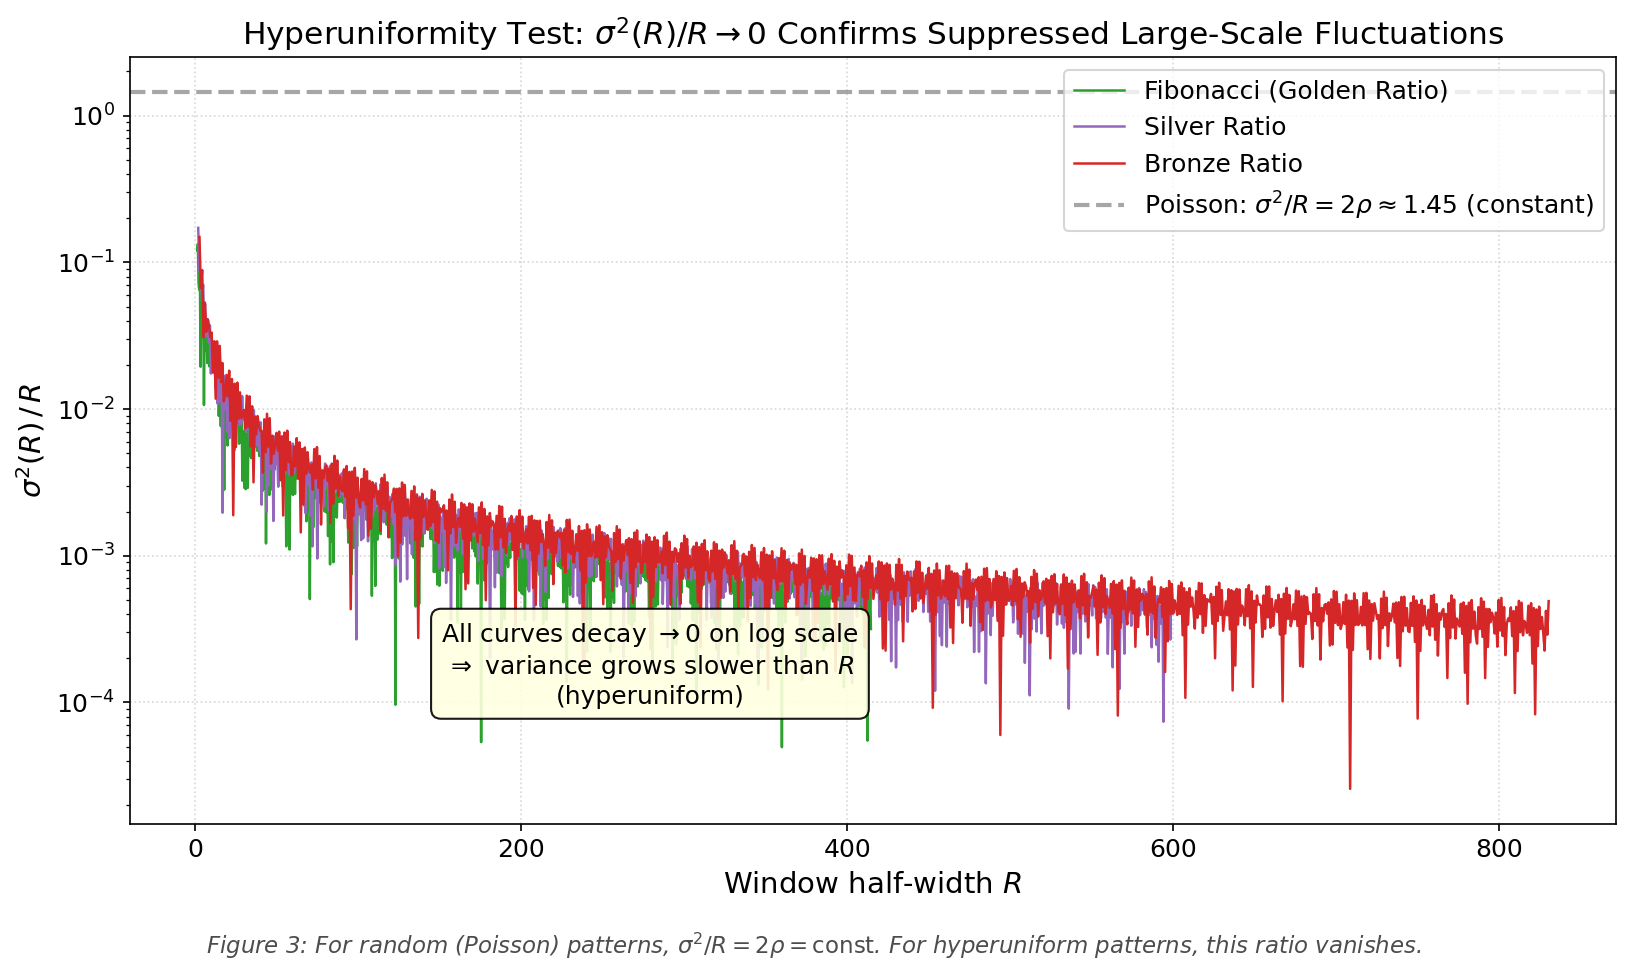
\includegraphics[width=0.8\textwidth]{../results/figures/fig3_hyperuniformity_test.png}
  \caption{Hyperuniformity test plot showing $\sigma^2(R)/(2\rho R)$ versus $R$ for
  selected patterns. Curves that approach zero confirm hyperuniformity; the horizontal
  Poisson baseline ($= 1$) serves as reference. Class~I patterns approach zero as $\sim
  1/R$, Class~II as $\sim \ln R / R$, and Class~III as $\sim R^{-\alpha}$.}
  \label{fig:hyperuniformity-test}
\end{figure}

\begin{figure}[H]
  \centering
  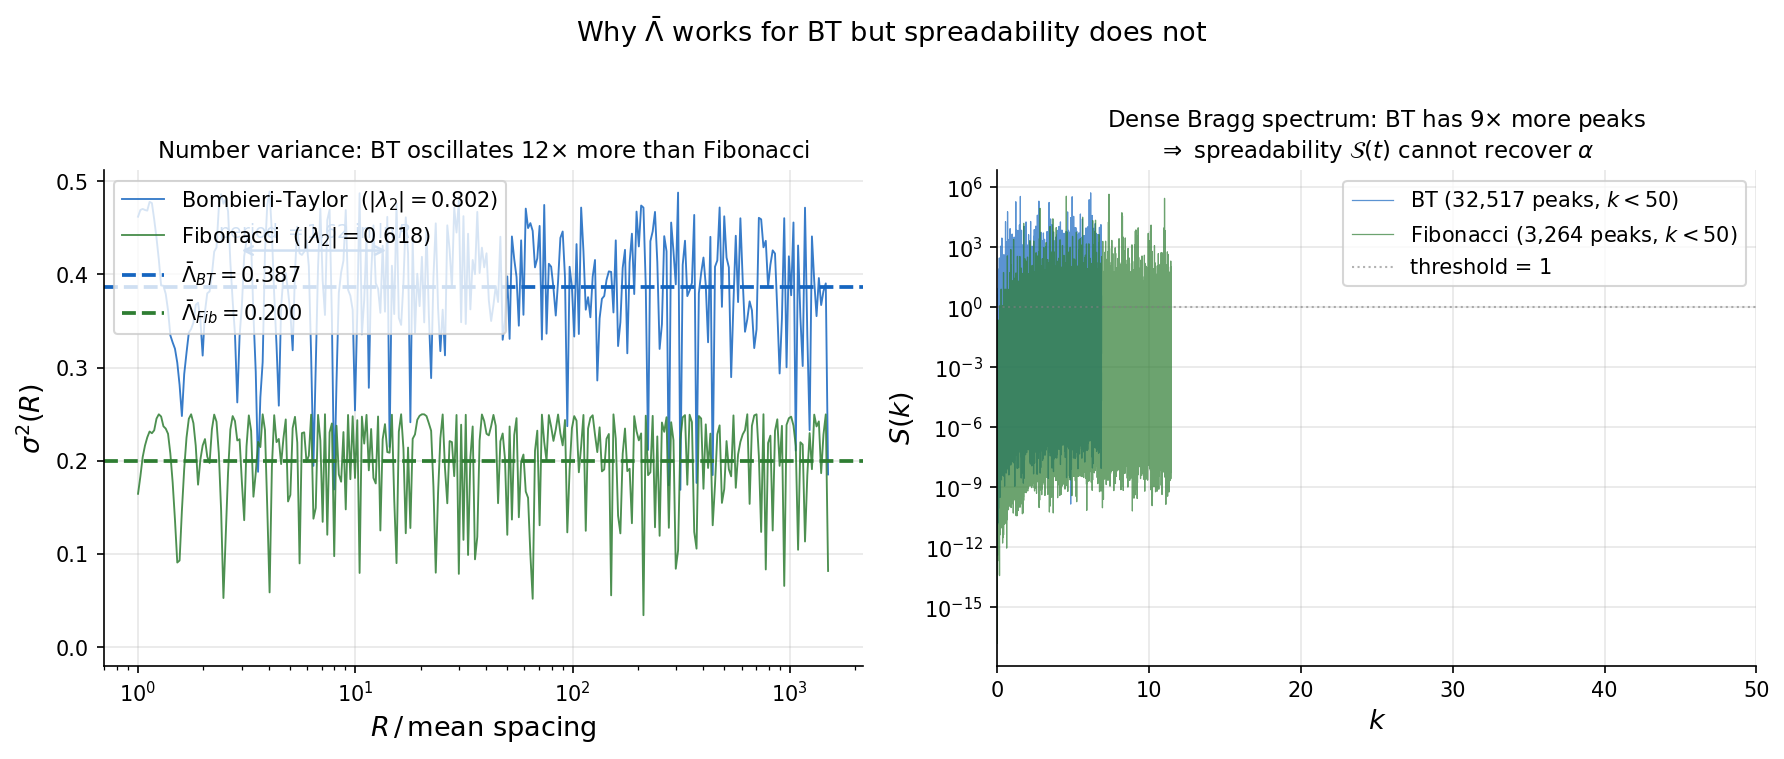
\includegraphics[width=0.95\textwidth]{../results/figures/fig_bt_deep.png}
  \caption{Bombieri-Taylor deep analysis. \textit{(a)} Fine-resolution number variance
  $\sigma^2(R)$ showing the strong log-periodic oscillations with period $2\ln\theta_1 \approx
  1.62$ in $\ln R$. \textit{(b)} Structure factor $S(k)$ over a wide $k$-range, revealing the
  dense Bragg peak spectrum (32,517 peaks in $k < 50$, compared to 2,637 for Fibonacci).
  \textit{(c,d)} Spreadability $\mathcal{S}(t)$ with standard and period-aware power-law fits.
  The large $|\lambda_2| = 0.802$ causes slow convergence; at $t \in [10^5, 10^9]$ the fit
  yields $\hat\alpha = 1.67$, still above the theoretical value 1.545.}
  \label{fig:bt-deep}
\end{figure}

\begin{figure}[H]
  \centering
  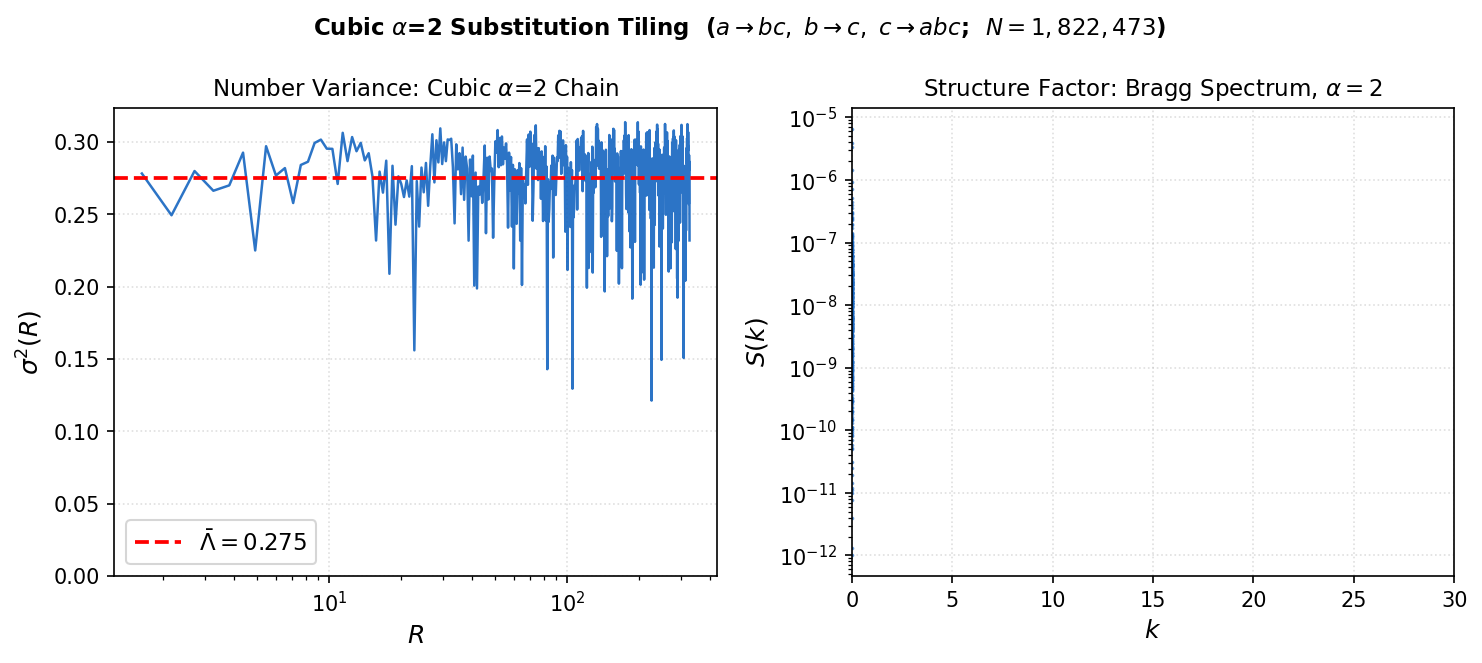
\includegraphics[width=0.9\textwidth]{../results/figures/fig_new_tilings.png}
  \caption{Hyperuniformity analysis of the cubic $\alpha$=2 substitution chain
  ($c \to abc$, $a \to bc$, $b \to c$; $N \approx 1.8 \times 10^6$).
  \textit{(Left)} Number variance $\sigma^2(R)$ is bounded (Class~I), saturating at
  $\bar\Lambda = 0.275$.
  \textit{(Right)} Structure factor shows the expected Bragg-peak spectrum, consistent
  with $\alpha = 2$ from Eq.~\eqref{eq:alpha2-proof}.}
  \label{fig:new-tilings}
\end{figure}

\begin{figure}[H]
  \centering
  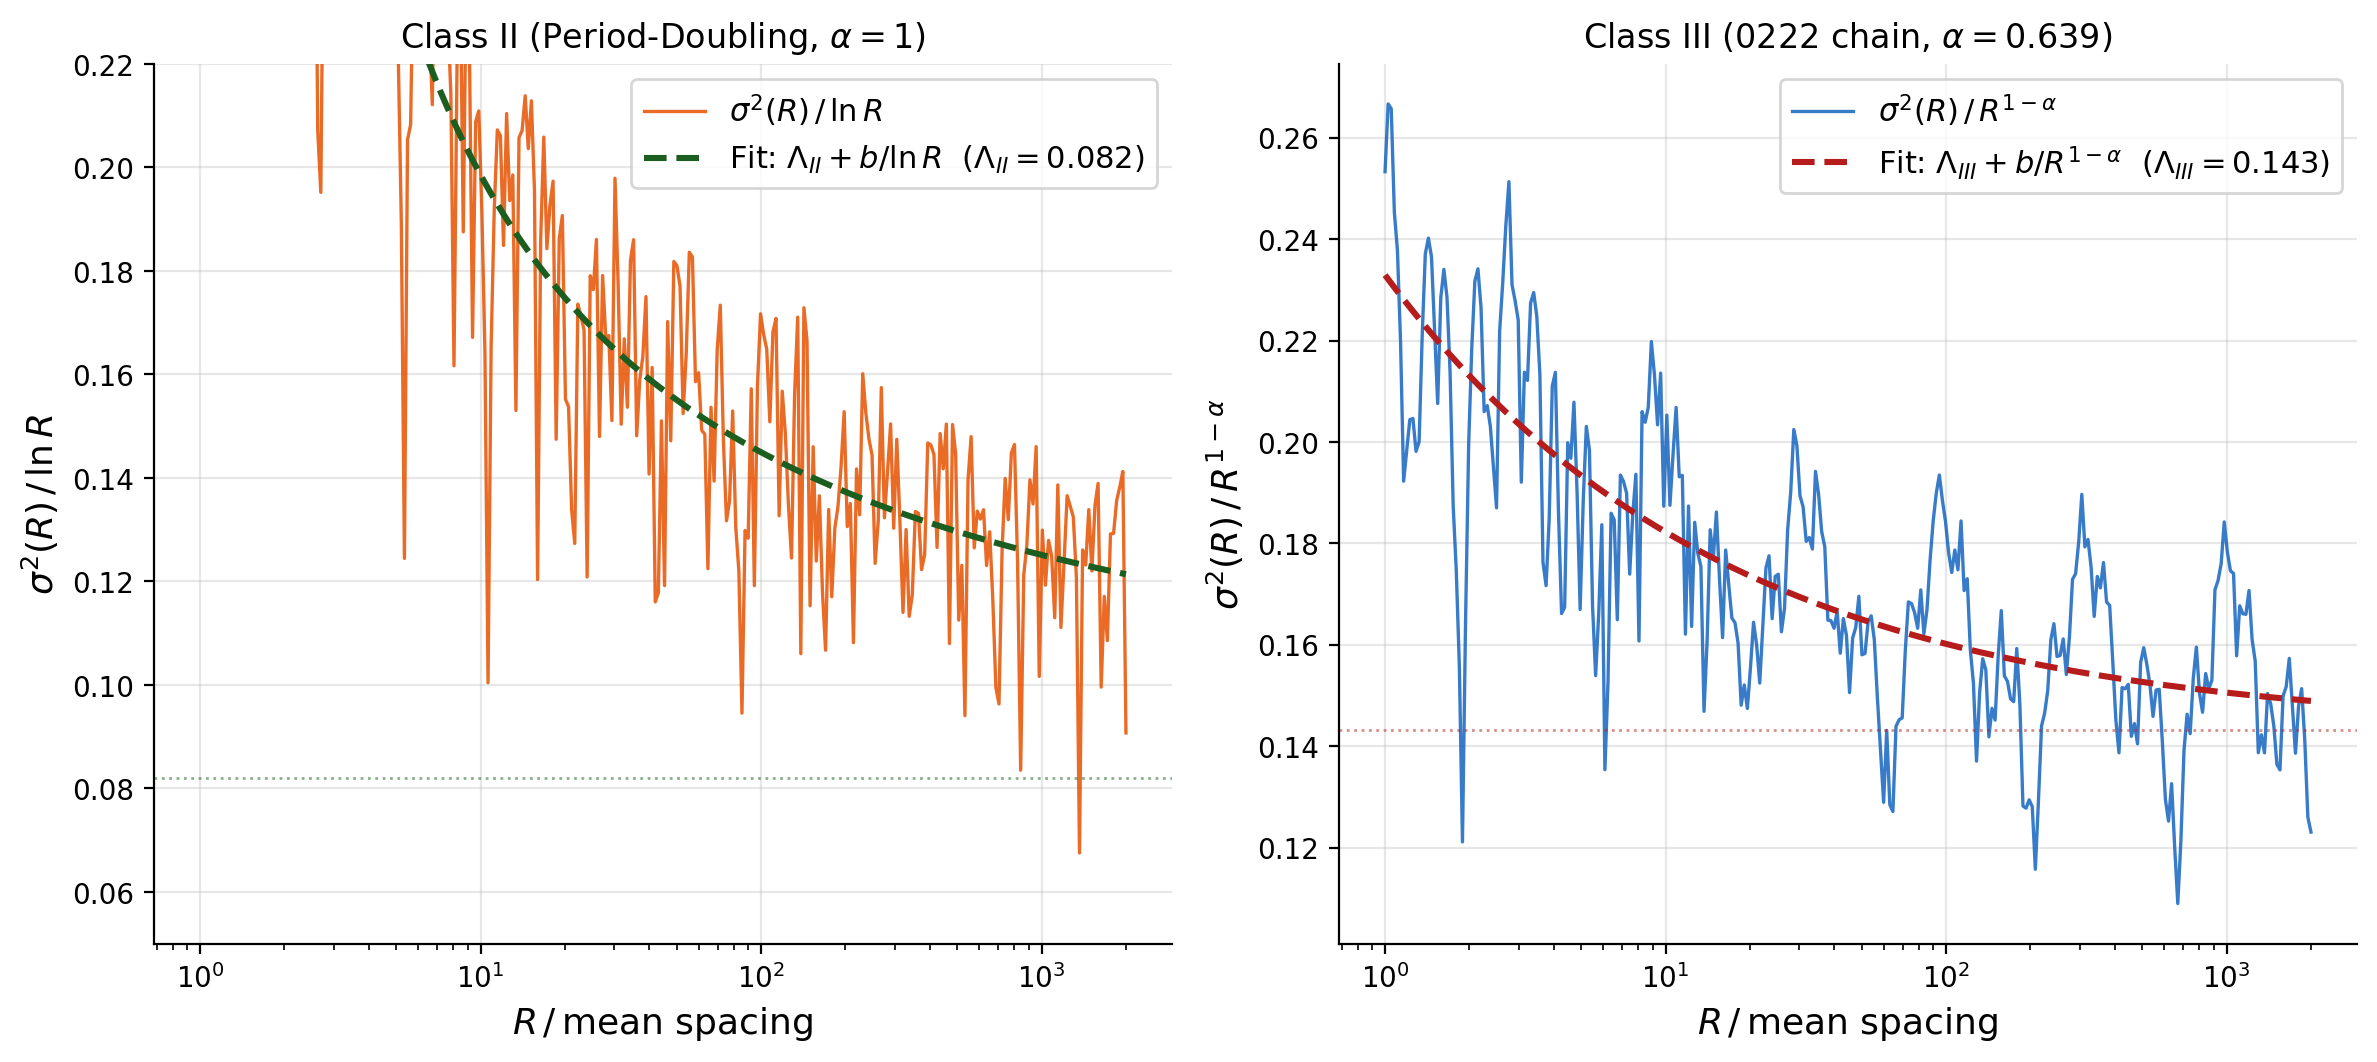
\includegraphics[width=0.9\textwidth]{../results/figures/fig_generalized_metrics.png}
  \caption{Generalized scaling metrics for Class~II and Class~III patterns.
  \textit{(Left)} Period-Doubling: normalized variance $\sigma^2(R)/\ln R$ approaches a
  constant $C_{II} = 0.123 \pm 0.016$ at large $R$, confirming the logarithmic scaling law.
  \textit{(Right)} 0222 chain: $\sigma^2(R)/R^{1-\alpha}$ (with $\alpha = 0.639$ from the
  eigenvalue formula) approaches $A_{III} = 0.151 \pm 0.014$, confirming the power-law
  scaling.}
  \label{fig:generalized-metrics}
\end{figure}

\begin{figure}[H]
  \centering
  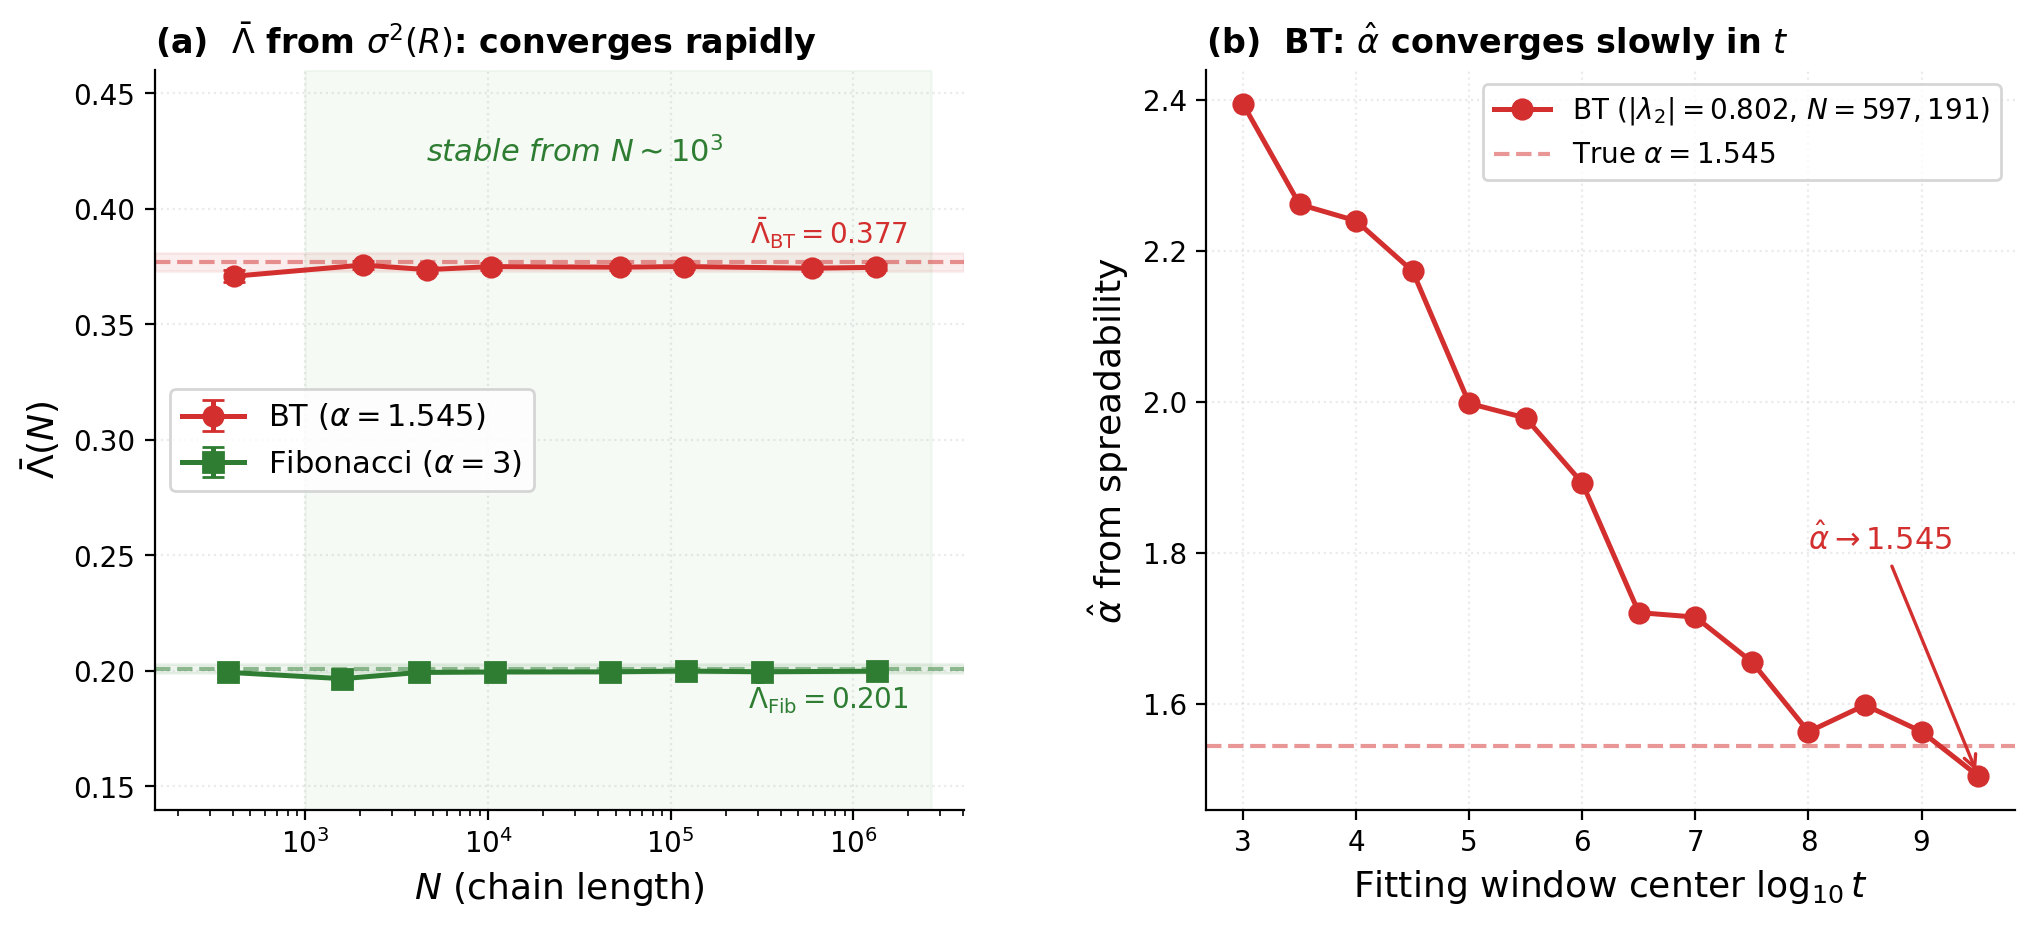
\includegraphics[width=0.9\textwidth]{../results/figures/fig_finite_size_alpha.png}
  \caption{Finite-size convergence of variance-based hyperuniformity metrics as a function of
  system size $N$. Class~I metrics ($\bar\Lambda$ for Bombieri-Taylor and Fibonacci) converge
  rapidly and are stable for $N \gtrsim 2000$. The Class~II metric $C_{II}$ for the
  period-doubling chain requires $N \gtrsim 10^5$ for reliable estimation. The Class~III
  exponent $\hat\alpha$ for the 0222 chain shows slow convergence due to $|\lambda_2| > 1$.}
  \label{fig:finite-size-alpha}
\end{figure}

\end{document}
